\pdfminorversion=7
\documentclass[utf8, english, usepdftitle=false, svgnames, color="table, fixpdftex, fixinclude, xcdraw", t]{beamer}


\usepackage{latexscholar-i18n}
\usepackage{latexscholar-quote}
\usepackage{latexscholar-verbatim}
\usepackage{lode-imacid}
\usepackage{lode-pdf}
\usepackage{multirow}

\usepackage{latexscholar-table}
\usepackage{tabularx}
\usepackage{multirow}

\usepackage{animate}
\usepackage{movie15}

\usepackage{inputx}
\inputpaths{../CommonAssets/}

\graphicspath{{../CommonAssets/}}


\title{Software testing}
\subtitle{Functional testing}
\author[]{%
Marco Aurelio Graciotto Silva\inst{1}, \\\and
}

\newcommand{\numberofinstitutes}{1}
\institute[UTFPR]
{
	\inst{1}%
	Federal University of Technology -- Parana (UTFPR)\\
	Campo Mourao, PR, Brazil
}
% \institute[ICMC]
% {
% 	\inst{2}%
% 	University of Sao Paulo (USP)\\
% 	Sao Carlos, SP, Brazil
% }


\date[]{February 2014}

% \logopicture{icmc-qualipso-inf}
% \logopicture{icmc-qualipso-inf}


\begin{document}

\frontmatter{}
\begin{frame}[c, plain]
\label{title}
\titlepage
\end{frame}

%\begin{frame}[c,parent={title}, hasprev=false, hasnext=false]
%\frametitle{Software Testing}
%\label{cmap:software-testing}
%
%\insertcmap{Courses-SoftwareTesting-SoftwareTesting}
%\end{frame}

\begin{frame}[c,parent={title}, hasprev=false, hasnext=false]
\frametitle{Software Testing}
\label{cmap:software-testing}

\centering
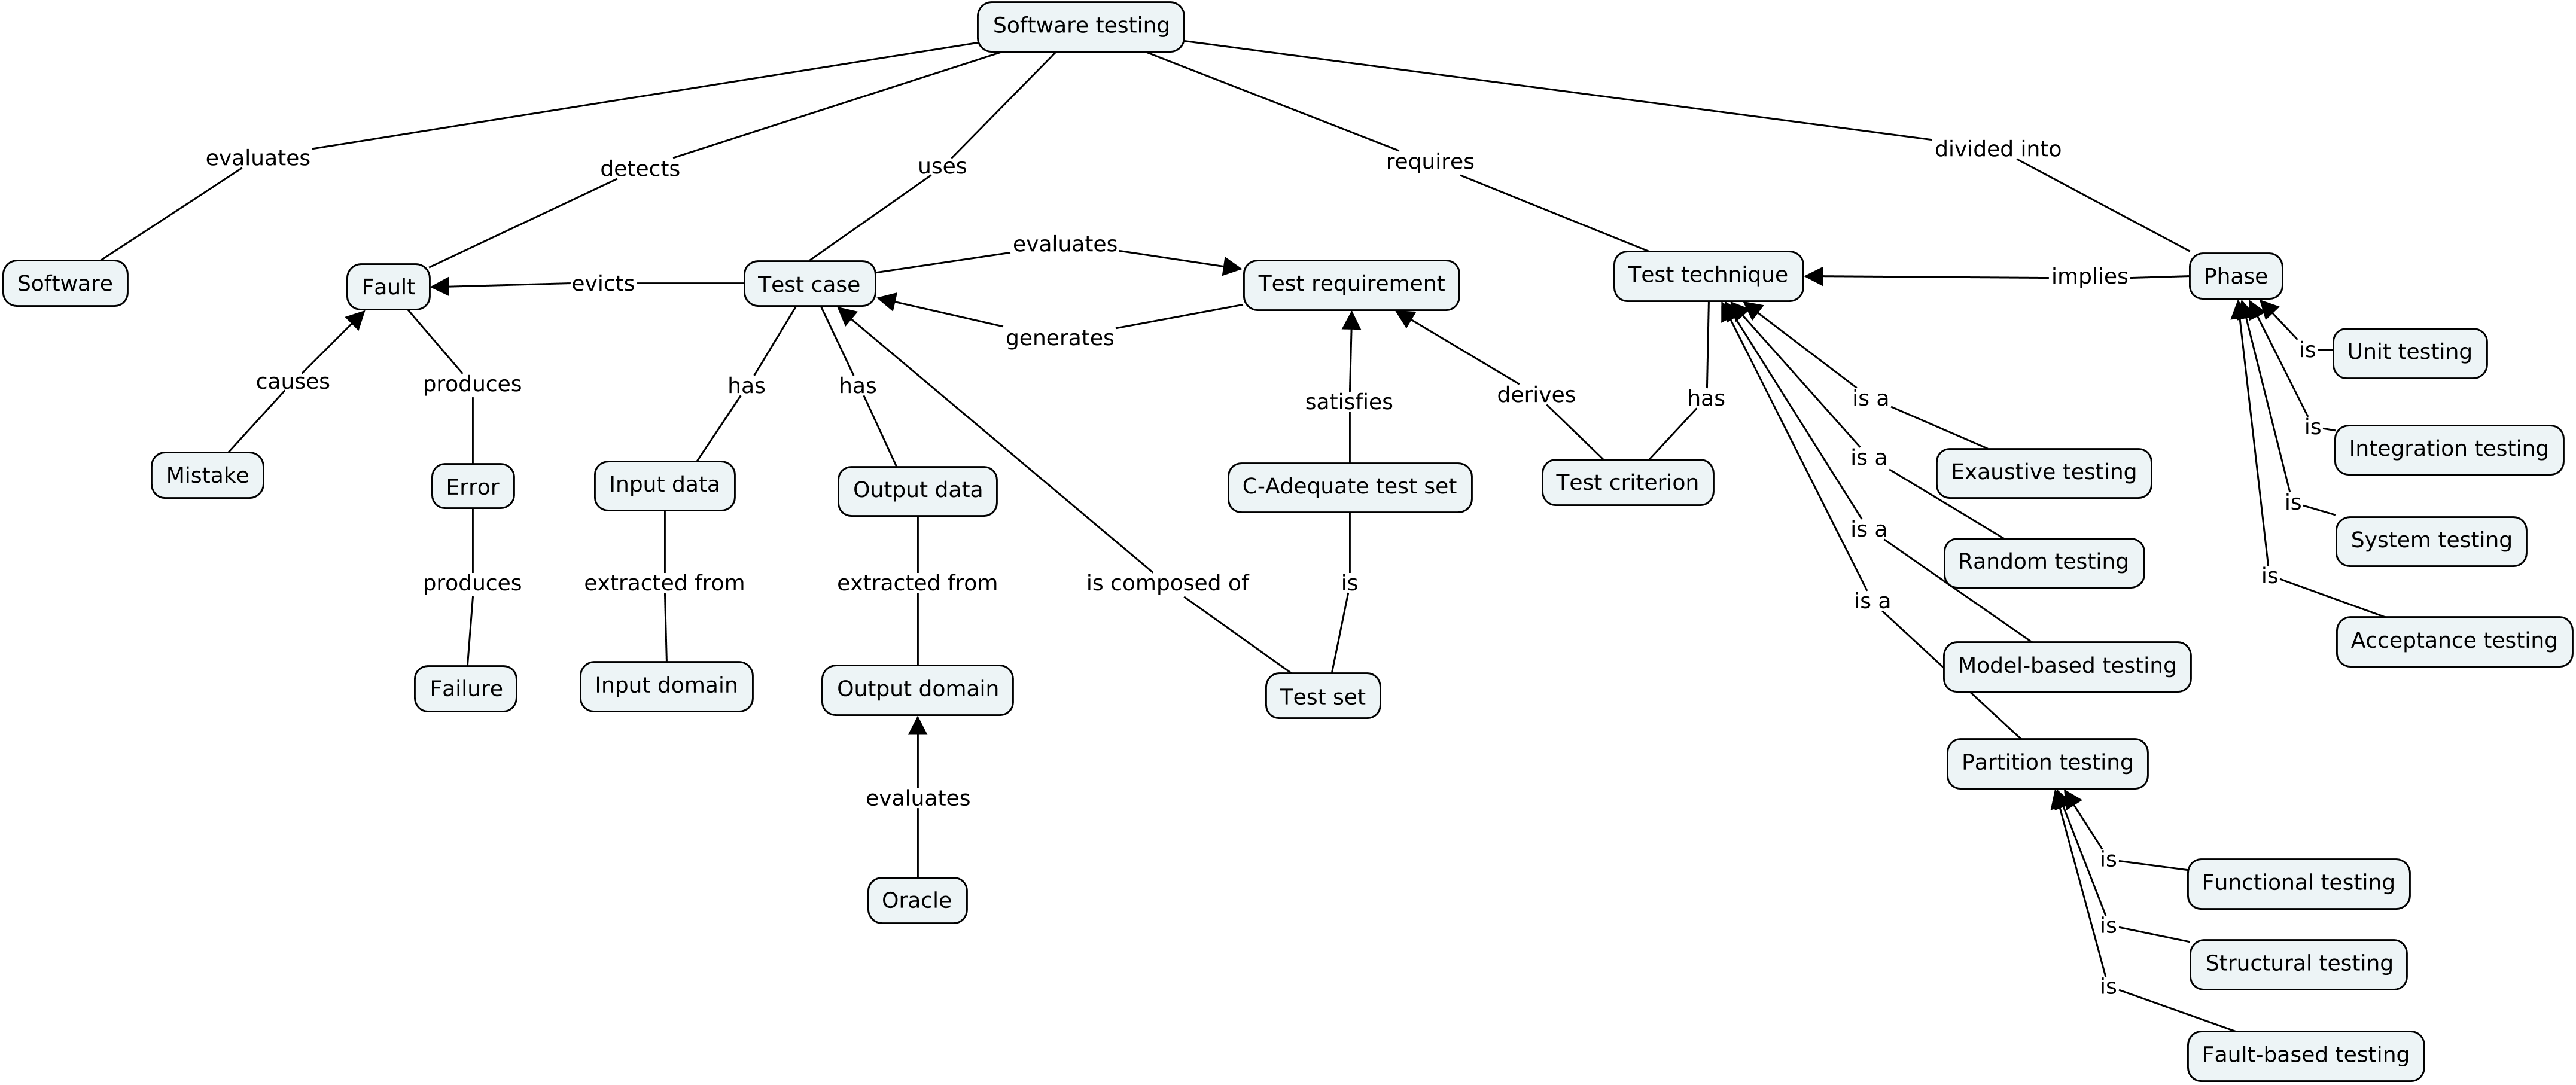
\includegraphics[width=\textwidth]{../BasicConcepts/Software testing fundamentals.png}
\end{frame}



\mainmatter{}
\part{Functional testing}
\section{Functional testing}
\begin{frame}[hasprev=false,hasnext=false]
\label{example:functional-testing}
\frametitle{Functional testing example}

Consider the function $x^y$, where $x$ is an integer and $y$ is a non-negative
integer. The input domain is: for every tuple (x,y), consider all possible values
of $x$ and $y >= 0$. The input domain can be partitioned as follows:

\begin{block:ie}{}
    \centering
    \includegraphics[width=4cm]{aux/examples/functional-testing/functional-testing}
\end{block:ie}
\end{frame}



\subsection{Equivalence partition}
\begin{frame}[hasprev=false, hasnext=true]
\frametitle{Equivalence partition example}

\begin{block:fact}{DIMENSION}
Assume that you are developing a compiler for a subset of Fortran and
that your team is currently implementing the statement
\srccode{DIMENSION}. The following requirements must be satisfied:

\begin{enumerate}
	\item The syntax of the \srccode{DIMENSION} statement is
	\srccode{DIMENSION ad[, ad]*}, where:
	\begin{itemize}
		\item \srccode{ad} is an array descriptor of the form
		\srccode{n(d[, d]*)},

		\item \srccode{n} is the symbolic name of the array,

		\item \srccode{d} is the dimension declarator.
	\end{itemize}

	\item Symbolic names can be one to six letters or digits, the first of
	which must be a letter.
\end{enumerate}
\end{block:fact}
\end{frame}


\begin{frame}[hasprev=false, hasnext=true]
\frametitle{Equivalence partition example}

\begin{block:fact}{DIMENSION}
\begin{enumerate}
	\item The minimum and maximum numbers of dimension declarations that can
	be specified for an array are 1 and 7, respectively.

	\item The syntax of a dimension declarator $d$ is \srccode{[lb: ]?ub}, where
	\srccode{lb} and \srccode{ub} are, respectively, the lower and upper
	dimension bounds.

	\item If no \srccode{lb} is specified, it is assumed to be one.

	\item The value of \srccode{ub} must be greater or equal to \srccode{lb}.

	\item The \srccode{DIMENSION} statement may be continued over multiple
	lines.
\end{enumerate}
\end{block:fact}
\end{frame}


\begin{frame}[hasprev=true, hasnext=true]
\frametitle{Equivalence partition example}
\framesubtitle{Classes}

\begin{block}{Equivalence classes form}
\begin{tabularx}{\textwidth}{|X|X|}
\textbf{Input condition}		& \textbf{Valid class}\\\hline
Number of array descriptors 	& one (1); more than one (2)\\\hline
Size of the array name			& 1-6 (4)\\\hline
Array name						& has letters (7); has digits (8)\\\hline
Array name starts with letter	& yes (10)\\\hline
Number of dimensions			& 1-7 (12)\\\hline
Lower bound is specified		& no (15); yes and it is a number (16)\\\hline
Upper bound is specified		& yes, and it is equal or greater than lower bound (18)\\\hline
Statement has multiple lines	& yes (22); no (23)\\
\end{tabularx}
\end{block}
\end{frame}




\begin{frame}[hasprev=true, hasnext=true]
\frametitle{Equivalence partition example}
\framesubtitle{Classes}

\begin{block}{Equivalence classes form}
\begin{tabularx}{\textwidth}{|X|X|}
\textbf{Input condition}		& \textbf{Invalid class}\\\hline
Number of array descriptors 	&  none (3) \\\hline
Size of the array name			&  0 (5), more than 6 (6)\\\hline
Array name						&  has something else (9)\\\hline
Array name starts with letter	&  no (11)\\\hline
Number of dimensions			&  0 (13), more than 7 (14)\\\hline
Lower bound is specified		&  yes, but it is not a number (17)\\\hline
Upper bound is specified		&  yes, but it is not a number (19); yes, but it is less than lower bound (20)\\\hline
Statement has multiple lines	&  -\\
\end{tabularx}
\end{block}
\end{frame}




\begin{frame}
\frametitle{Equivalence partition example}
\framesubtitle{Test cases}

\begin{block}{Test cases and classes}
\begin{itemize}
	\item For each test case, the test requirements (equivalence classes) that
	they cover are in bold face.
	\begin{itemize}
		\item One single test case can cover several valid classes.

		\item There must have one test case for each invalid class.
	\end{itemize}
\end{itemize}
\end{block}


\begin{block}{Test cases for valid classes}
\begin{itemize}
	\item \srccode{DIMENSION A(2)} \textbf{(1, 4, 7, 23)}
	\item \srccode{DIMENSION A 12345(9, 100),}\\\srccode{BBB(-15:30)} \textbf{(2, 8, 16, 18, 22)}
	\item \srccode{DIMENSION D(:1)} \textbf{(15)}
\end{itemize}
\end{block}
\end{frame}


\begin{frame}[hasprev=true, hasnext=false]
\frametitle{Equivalence partition example}
\framesubtitle{Test cases}

\begin{block}{Test cases for invalid classes}
\begin{itemize}
	\item \srccode{DIMENSION} \textbf{(3)}
	\item \srccode{DIMENSION (10)} \textbf{(5)}
	\item \srccode{DIMENSION A234567(2)} \textbf{(6)}
	\item \srccode{DIMENSION A.1(2)} \textbf{(9)}
	\item \srccode{DIMENSION 1A(10)} \textbf{(11)}
	\item \srccode{DIMENSION B} \textbf{(13)}
	\item \srccode{DIMENSION B(1, 2, 3, 4, 5, 6, 7, 8)} \textbf{(14)}
	\item \srccode{DIMENSION B(ABC)} \textbf{(17)}
	\item \srccode{DIMENSION C(4:ABC)} \textbf{(19)}
	\item \srccode{DIMENSION C(4:3)} \textbf{(20)}

\end{itemize}
\end{block}
\end{frame}

\subsection{Boundary value analysis}
\begin{frame}[hasprev=false, hasnext=true, parent={concept:functional-testing}]
\frametitle{Boundary value analysis}

\begin{block:fact}{}
\begin{itemize}
	\item Experience shows that test cases that explore \textbf{boundary
	conditions} have a higher payout than test cases that do
	not~\cite[p.~59]{Myers:2004}.

	\item Hence it would be interesting to have a test criterion that
	exploits such situations.
\end{itemize}
\end{block:fact}
\end{frame}


\begin{frame}[hasprev=true, hasnext=true]
\frametitle{Boundary value analysis}
\label{concept:boundary-value-analysis}

\begin{block:concept}{Boundary value analysis}
Boundary value analysis requires that test cases be selected based on the
boundaries of each equivalence class.
\end{block:concept}

\begin{block:fact}{Boundary value analysis and equivalent partition}
\begin{itemize}
	\item Boundary value analysis is complementary to equivalent partition.

	\item It explores boundary conditions, such as the same, above and below
	limits in the equivalence class.
\end{itemize}
\end{block:fact}
\end{frame}


\begin{frame}
\frametitle{Boundary value analysis}
\framesubtitle{Boundary for a range}

\begin{block:fact}{Boundary for a range}
\begin{itemize}
	\item The input for a test case for an input which boundary conditions
	establish a range of values must be:
	\begin{itemize}
		\item in the limits of the range,
		\item above and below the limits.
	\end{itemize}
\end{itemize}
\end{block:fact}
\end{frame}


\begin{frame}
\frametitle{Boundary value analysis}
\framesubtitle{Boundary for a range}

\begin{block}{Example of boundaries for a range}
\begin{itemize}
	\item The requirement states that ``the item count can be from 1 to 999''.

	\item There are three equivalence classes:
	\begin{itemize}
		\item Valid class: item count between 1 and 999 (including the number
		1 and 999).
		\item Invalid classes:
		\begin{itemize}
			\item item count with a value less than 1
			\item item count with a value greater than 999.
		\end{itemize}
	\end{itemize}

	\item The values to be tested are:
	\begin{itemize}
		\item 0 (just below/out the range)
		\item 1 (just in the range considering the lower limit)
		\item 999 (just in the range considering the upper limit)
		\item 1000 (just above/out the range)
	\end{itemize}
\end{itemize}
\end{block}
\end{frame}



\begin{frame}
\frametitle{Boundary value analysis}
\framesubtitle{Boundary for a sequence}

\begin{block:fact}{Boundary for a sequence}
\begin{itemize}
	\item The input of a test case for an input which boundary conditions
	establish a sequence of values must be:
	\begin{itemize}
		\item in the limit,
		\item and one unit below and above the limit.
	\end{itemize}
\end{itemize}
\end{block:fact}
\end{frame}


\begin{frame}
\frametitle{Boundary value analysis}
\framesubtitle{Boundary for a sequence}

\begin{block}{Example}
\begin{itemize}
	\item The requirement states that ``one throught six owners can be listed
	for the automobile''.

	\item There are three equivalence classes:
	\begin{itemize}
		\item Valid class: list of owners with one to six names.
		\item Invalid classes:
		\begin{itemize}
			\item empty owner list,
			\item owner list with more than six names.
		\end{itemize}
	\end{itemize}

		\item The values to be tested are:
	\begin{itemize}
		\item 0 (one unit below the limit)
		\item 1 (just in the limit considering the lower limit)
		\item 5 (just in the limit considering the upper limit)
		\item 7 (one unit above the limit)
	\end{itemize}
\end{itemize}
\end{block}
\end{frame}


\begin{frame}[hasprev=true, hasnext=false]
\frametitle{Boundary value analysis}
\framesubtitle{Limitations}

\begin{block:fact}{Limitations}
\begin{itemize}
	\item Boundary value analysis does not explore input condition combinations.
\end{itemize}
\end{block:fact}
\end{frame}

\subsection{Cause effect graph}
\begin{frame}[parent={concept:functional-testing}, hasprev=false, hasnext=true]
\frametitle{Cause-effect graph}
\label{concept:case-effect-graph}

\begin{block:concept}{Cause-effect graph}
Cause-effect graph establishes test requirements based on the possible
combinations of input conditions.
\end{block:concept}


\begin{block:fact}{Input conditions combination}
\begin{itemize}
	\item You could combine and select input conditions and test such
	combinations using equivalence partition.

	\item However, as the number of possible combinations is usually high,
	it is likely that the subsets of combinations to be tested will be chosen
	arbitrarily.
	\begin{itemize}
		\item This would lead to an ineffective test.
	\end{itemize}

	\item Cause-effect graphing aids in selecting, in a systematic way,
	a high yield set of test cases~\cite[p.~66]{Myers:2004}.
\end{itemize}
\end{block:fact}
\end{frame}


\begin{frame}[hasprev=true, hasnext=true]
\frametitle{Cause-effect graph}

\begin{block:fact}{Cause-effect graph}
The cause-effect graph creates a boolean graph that is a formal
language to describe the software specification.
\end{block:fact}


\begin{block:fact}{Cause}
In the cause-effect graph, the causes corresponds to:
\begin{itemize}
	\item input conditions of a given equivalence classes,
	\item stimulus,
	\item or anything else that causes an output of the program under
	testing.
\end{itemize}
\end{block:fact}


\begin{block:fact}{Effect}
In the cause-effect graph, the effects are:
\begin{itemize}
	\item the output,
	\item system state changes, or
	\item any observable outcome.
\end{itemize}
\end{block:fact}
\end{frame}


\begin{frame}
\frametitle{Cause-effect graph}

\begin{block:procedure}{How to create the graph}
\begin{enumerate}
	\item Identify the possible input conditions (causes) and the possible
	actions of the product (effects).
	\begin{itemize}
		\item Hint: equivalence classes are a cause.
		\item Associate an unique identifier for each cause and effect found
		(a numeric id is fine).
	\end{itemize}

	\item Build a cause-effect graph by relating causes with identified
	effects.

    \item Impossible cause-effect combinations must be annotated in the graph.
\end{enumerate}
\end{block:procedure}
\end{frame}


\begin{frame}
\frametitle{Cause-effect graph}

\begin{block:fact}{Cause-effect graph elements}
\begin{itemize}
	\item Each node in the graph represents a input condition (cause) and
	outcomes (effects).

	\item Each node can be assigned the value 0 or 1.
	\begin{itemize}
		\item 0 represents the ``absent'' state.
		\item 1 represents the ``present'' state.
	\end{itemize}

	\item The relationships between the nodes is represented using the
	functions:
	\begin{itemize}
		\item identity,
		\item not,
		\item or,
		\item and.
	\end{itemize}
\end{itemize}
\end{block:fact}
\end{frame}


\begin{frame}
\frametitle{Cause-effect graph}


\begin{columns}[t]
\column{.4\textwidth}
\begin{block:fact}{Unary boolean functions}
\begin{tabular}{l|c|c}
\textbf{Function}			& \textbf{A}	& \textbf{Result}\\\hline\hline
\multirow{2}{*}{Identity} 	& 0 			& 0\\
							& 1 			& 1\\\hline\hline
\multirow{2}{*}{Not}		& 0 			& 1\\
							& 1				& 0\\
\end{tabular}
\end{block:fact}

\qquad
\column{.5\textwidth}
\begin{block:fact}{N-ary boolean functions}
\begin{tabular}{l|c|c|c}
\textbf{Function}			& \textbf{A}	& \textbf{B}	& \textbf{Result}\\\hline\hline
\multirow{4}{*}{Or} 		& 0 			& 0				& 0\\
							& 0 			& 1				& 1\\
							& 1 			& 0				& 1\\
							& 1 			& 1				& 1\\\hline\hline
\multirow{4}{*}{And}		& 0 			& 0				& 0\\
							& 0 			& 1				& 0\\
							& 1 			& 0				& 0\\
							& 1 			& 1				& 1\\
\end{tabular}
\end{block:fact}
\end{columns}

\end{frame}



\begin{frame}
\frametitle{Cause-effect graph}

\begin{block}{Function symbols}
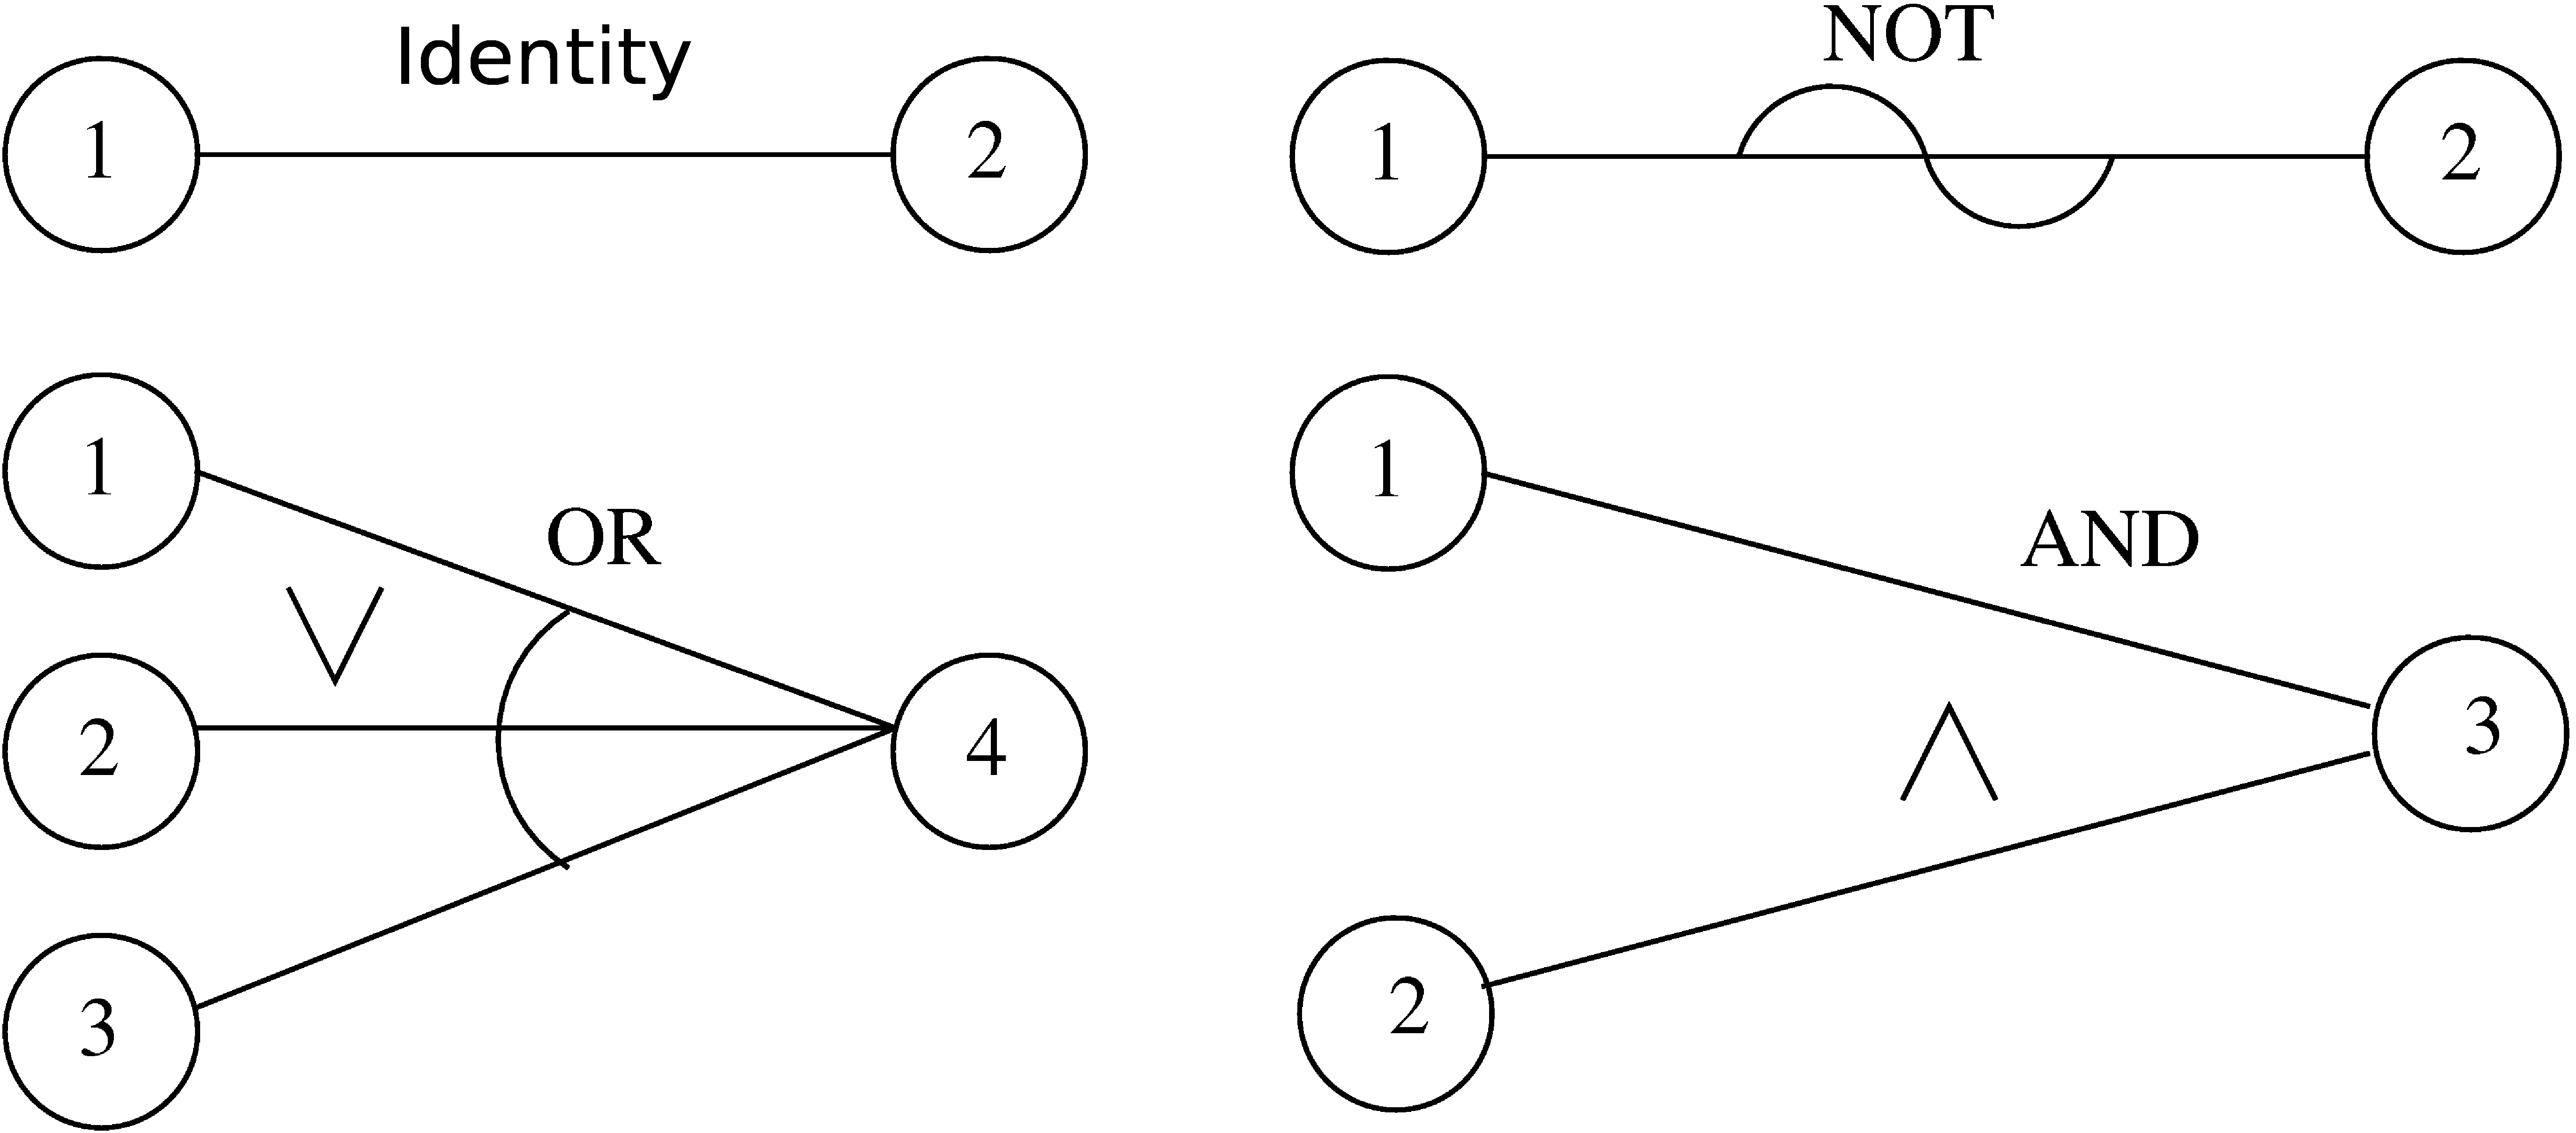
\includegraphics[scale=.04]{Functional testing/Cause-effect graph/Cause-effect graph symbols}
\end{block}

\begin{block}{Restrictions symbols}
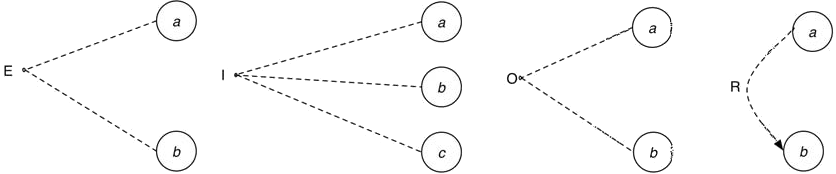
\includegraphics[width=\textwidth]{Functional testing/Cause-effect graph/Cause-effect graph restrictions}
\end{block}

\end{frame}





\begin{frame}
\frametitle{Cause-effect graph}
\label{procedure:cause-effect-graph}

\begin{block:procedure}{How to create the graph}
\begin{enumerate}
	\item To verify if the cause-effect graph is correct, it must be assigned
	the values 0 and 1 to the causes and check if the effects have the
	correct values.
\end{enumerate}
\end{block:procedure}


\hfill
\refie{example:cause-effect-graph}{\beamerbutton{Example}}
\end{frame}



\begin{frame}
\frametitle{Cause-effect graph}

\begin{block:procedure}{How to create the decision table}
\begin{enumerate}
	\item Convert the cause-effect graph into a decision table (from where test
	cases are derived).
	\begin{enumerate}
		\item Select an effect that should have the value 1.

		\item Trace back the cause-effect graph from the chosen effect, finding
		every cause combination that makes the effect have the value of 1.
		\begin{enumerate}
				\item In the cause-effect graph, if a node is of the OR-type
				and the output must be 1, never assign more than one input with
				the value 1 simultaneously.

				\item In the cause-effect graph, if a node is of the AND-type
				and the output must be 0, all the input combinations that
				returns an output of 0 must be enumerated. However, if one of
				the input is 0 and one or more of the input is 1, it is not
				necessary to enumerate all the conditions which input are
				equal to 1.
		\end{enumerate}
	\end{enumerate}
\end{enumerate}
\end{block:procedure}
\end{frame}


\begin{frame}
\frametitle{Cause-effect graph}

\begin{block:procedure}{How to create the decision table}
\begin{enumerate}
	\item (continuation) Convert the cause-effect graph into a decision table
	(from where test cases are derived).
	\begin{enumerate}
		\item Create a column in the decision table for every cause
		combination.

		\item Specify, for every cause combination, the state of every single
		effect, annotating them in the table.
	\end{enumerate}
\end{enumerate}
\end{block:procedure}
\end{frame}


% \begin{frame}[hasprev=true, hasnext=false]
% \frametitle{Cause-effect graph}
%
% \begin{block:fact}{}
% \begin{itemize}
% 	\item The definition of the cause-effect graph helps to point out
% 	incompleteness and ambiguities in the software requirement
% 	specification~\cite[p. 66]{myers:2004}.
% \end{itemize}
% \end{block:fact}
% \end{frame}




\backmatter{}
\part{References and credits}
\include{bibliography}
\part{Acknowledgement}
\section*{Acknowledgement}


\begin{frame}[c,label=credits]
\frametitle{Credits}

\centering
\animategraphics[height=140pt,poster=first,autoplay,loop]{1}{main/jabuti-}{0}{3}

\begin{itemize}
	\item Reviewers:
	\begin{itemize}
		% \item Auri Marcelo Rizzo Vincenzi
		% \item Ellen Francine Barbosa
		\item Fabiano Cutigi Ferrari
		% \item Márcio Eduardo Delamaro
		\item Otávio Augusto Lazzarini Lemos
	\end{itemize}
\end{itemize}
\end{frame}


\part{Instructional elements}
\include{examples}
\include{exercises}


\end{document}
